\documentclass{scrreprt}
\usepackage{listings}
\usepackage{underscore}
\usepackage[bookmarks=true]{hyperref}
\usepackage[utf8]{inputenc}
\usepackage[english]{babel}
\usepackage{graphicx}
\graphicspath{{work_packages/work_package_1/static/user-manual-images/}} % path relative to root
%\graphicspath{{static/user-manual-images/}}
\hypersetup{
    pdftitle={Users Manual},    % title
    pdfauthor={Training Montage},                     % author
    pdfsubject={TeX and LaTeX},                        % subject of the document
    pdfkeywords={TeX, LaTeX, graphics, images}, % list of keywords
    colorlinks=true,       % false: boxed links; true: colored links
    linkcolor=blue,       % color of internal links
    citecolor=black,       % color of links to bibliography
    filecolor=black,        % color of file links
    urlcolor=purple,        % color of external links
    linktoc=page            % only page is linked
}

\def\myversion{0.1 }
\date{}

\usepackage{hyperref}
\begin{document}

\begin{flushright}
    \rule{16cm}{5pt}\vskip1cm
    \begin{bfseries}
        \Huge{USER'S MANUAL}\\
        \vspace{.9cm}
        for\\
        \vspace{.9cm}
        COE 1186 Project\\
        \vspace{.9cm}
        \LARGE{Version \myversion approved}\\
        \vspace{.9cm}
        Prepared by:\\
        Alec Rosenbaum\\
        Aric Hudson\\
        Isaac Goss\\
        Mitch Moran\\
        Parth Dadhania\\
        \vspace{1.9cm}
        Training Montage\\
        \vspace{.9cm}
        \today\\
    \end{bfseries}
\end{flushright}

\tableofcontents


%%%%%%%%%%%%%%%%%%   CTC Start   %%%%%%%%%%%%%%%%%%%%%
\chapter{Centralized Traffic Control}
\Large{Mitch Moran}\\

% picture(s) of overall gui
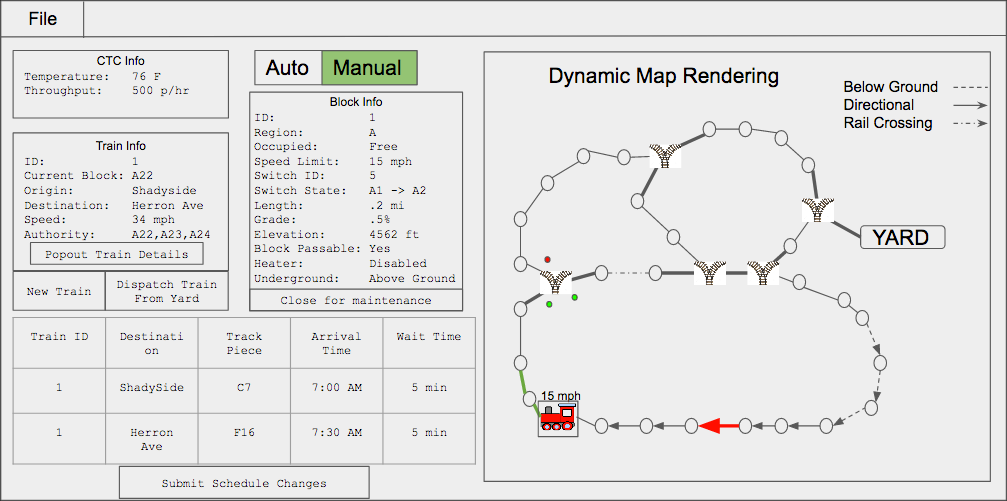
\includegraphics[width=\textwidth]{CTC-main}

\section{File Menu}
Clicking on file will show a drop down menu containing the following items:
\begin{itemize}
  \item Upload Schedule - Replace the existing schedule with a newly uploaded one
  \item Save Schedule - Export schedule with any manual changes to a file
  % Do I need an upload track option
\end{itemize}

\section{Auto/Manual Button}
\begin{center}
  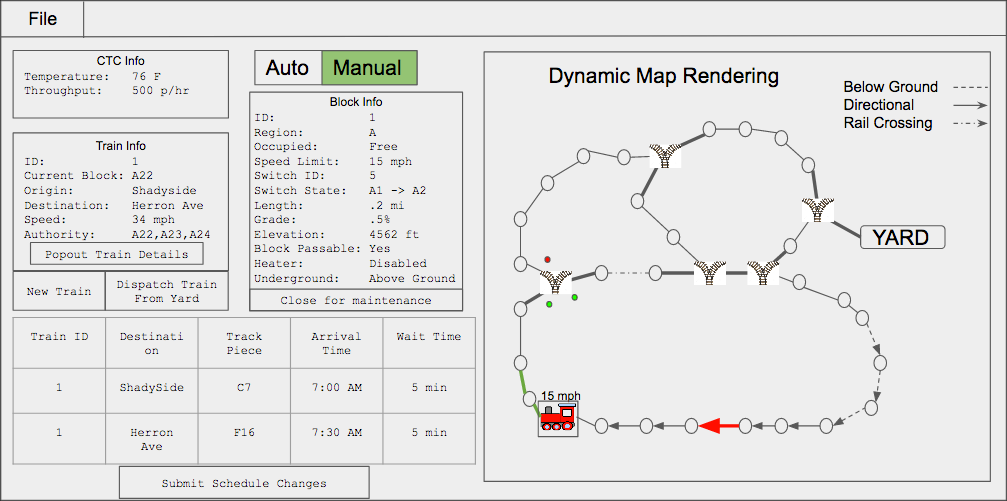
\includegraphics[trim={9cm 14.65cm 20.8cm 1.7cm},clip,width=3cm]{CTC-main}
\end{center}
% trim={<left> <lower> <right> <upper>}
Toggle between automatic and manual modes by clicking this button. In automatic mode trains
will be dispatched according to the internal schedule. In manual mode the dispatcher must
deploy all trains.

\section{Dynamic Map Rendering}
\begin{center}
  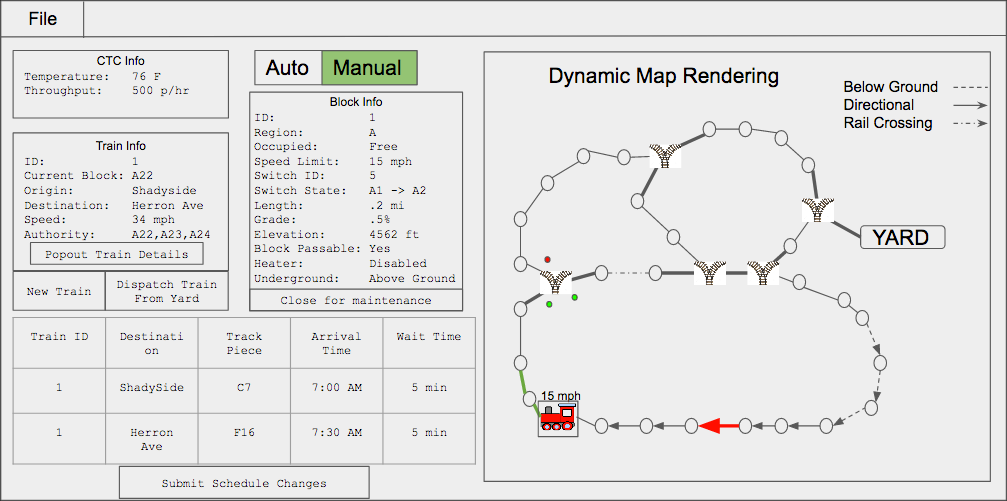
\includegraphics[trim={17cm .65cm .5cm 1.75cm},clip,width=\textwidth]{CTC-main}
\end{center}
% trim={<left> <lower> <right> <upper>}
The dynamic map rendering displays the current system state. Detailed information of each
piece will be displayed in the relevant info boxes when a train or piece of track is clicked.

\section{CTC Info}
\begin{center}
  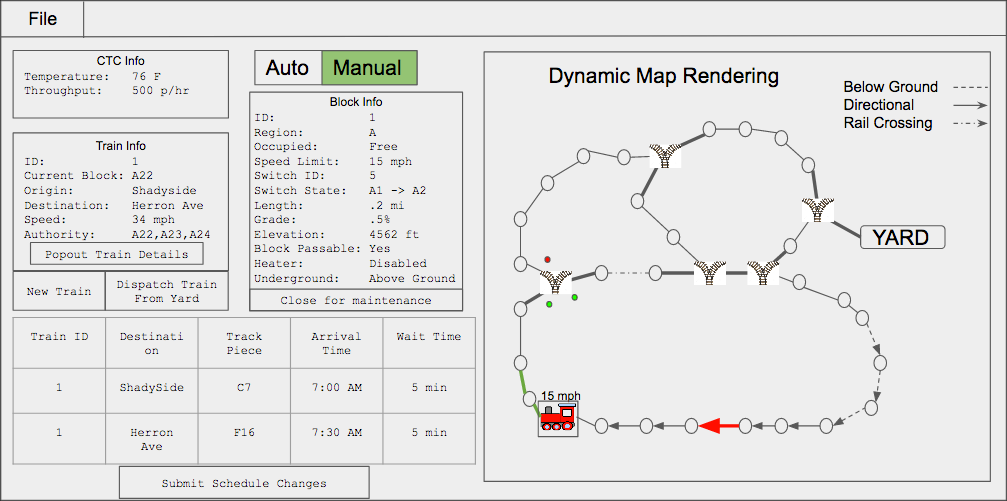
\includegraphics[trim={.45cm 13.5cm 27.45cm 1.7cm},clip,width=5cm]{CTC-main}
\end{center}
% trim={<left> <lower> <right> <upper>}
The CTC info box displays information about the currently operating system.
\begin{itemize}
  \item Temperature - Current outside temperature.
  \item Throughput - Amount of people that completed a trip within the last hour
\end{itemize}

\section{Train Info}
\begin{center}
  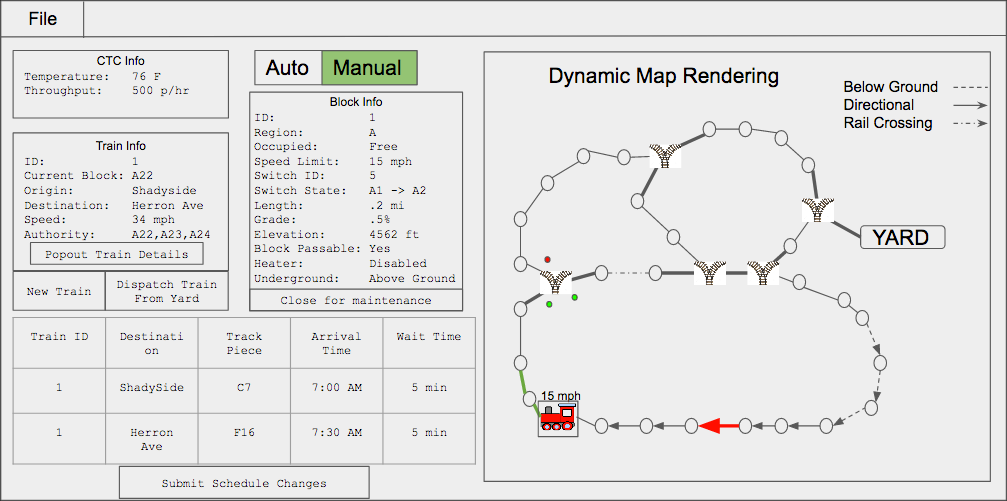
\includegraphics[trim={.45cm 6.6cm 27.45cm 4.6cm},clip,width=5cm]{CTC-main}
\end{center}
% trim={<left> <lower> <right> <upper>}
Information on a train selected in the map view will display here. The following items
will be displayed.
\begin{itemize}
  \item Train ID - Unique ID number for the train
  \item Current Block - The current block this train occupies
  \item Origin - Location the train started at
  \item Destination - Final stop for this train
  \item Speed - Speed suggested by the CTC
  \item Authority - The permitted distance until the train must stop
\end{itemize}
The Pop-out Train Details button will open a new window to allow the viewing of multiple
trains at once. This window will be explained in a later section. In manual mode, the New
Train button will create a blank template for the dispatcher to add a new train. Once the
new train's details are entered, Dispatch Train From Yard will send the new train. Closing
the template window without pressing the Dispatch button will cancel the new train.

\section{Block Info}
\begin{center}
  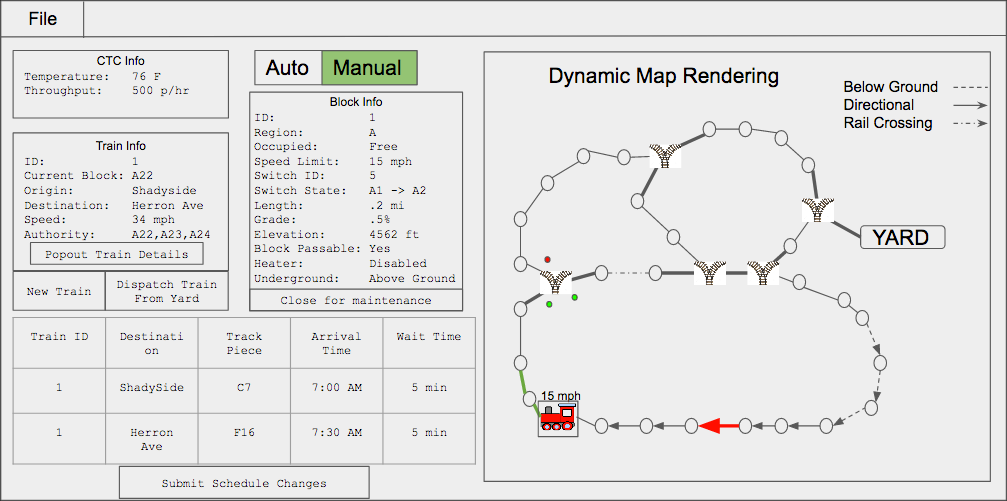
\includegraphics[trim={8.75cm 6.7cm 19.2cm 3.2cm},clip,width=5cm]{CTC-main}
\end{center}
% trim={<left> <lower> <right> <upper>}
Information on a block selected in the map view will display here. The following items
will be displayed. Items marked with an asterisk (*) are contextual and only appear when
relevant.
\begin{itemize}
  \item Block ID - Together with Region forms a unique block ID
  \item Region - The region of track in which this block is located
  \item Occupied - (Yes, No) Indicates if the block is occupied or not
  \item Speed Limit - The max safe speed for that block
  \item Length - How long the block is
  \item Grade - The grade of the block
  \item Elevation - The block's elevation
  \item Block Passable - (Yes, Broken, Maintenance) If the block can be passed or the reason
  it can't be passed
  \item Heater State - (On, Off, N/A) Indicates if the heater is on, off, or there is no heater
  \item Underground - (Yes, No) Indicates if the block is underground
  \item Light State* - (Super Green, Green, Yellow, Red) The light color currently displayed
  \item Switch ID* - A unique ID for the switch on this block
  \item Switch State* - Shows which track pieces are connected by a switch
  \item Station Name* - The name of the station on that block
  \item Number of Passengers at Station* - How many passengers are waiting at that station
  \item Railway Crossing State* - (Activated, Deactivated) When activated, trains can safely cross
\end{itemize}
The selected block can be closed or opened for maintenance by clicking the button at the
bottom of this box.

\section{Schedule}
\begin{center}
  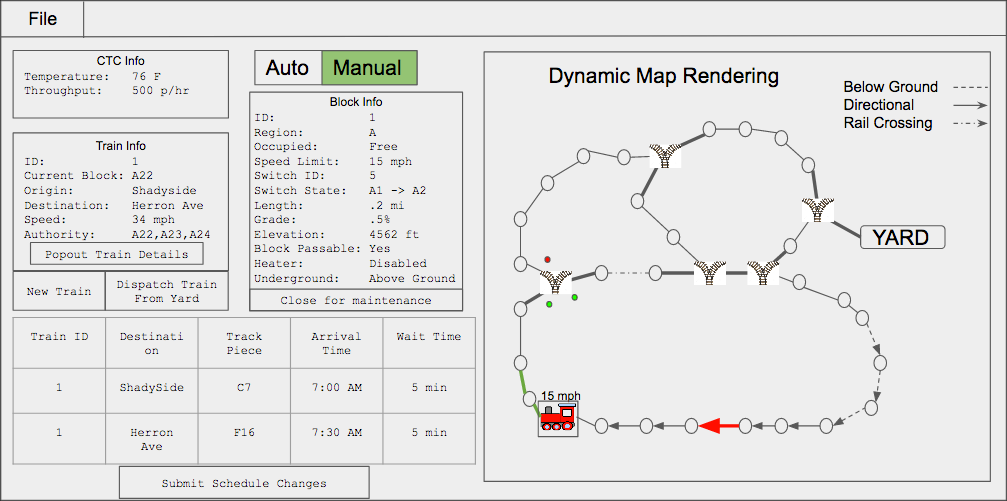
\includegraphics[trim={.45cm .08cm 18.7cm 11.15cm},clip,width=11cm]{CTC-main}
\end{center}
% trim={<left> <lower> <right> <upper>}
Displays the schedule for the whole system. Will be read-only in automatic mode and can be
edited in manual mode. Users can select a station from the Destination column or select a specific
block from the Track Piece column. Use the Submit button to confirm changes made to the schedule.

\section{Train Details Pop-out}
\begin{center}
  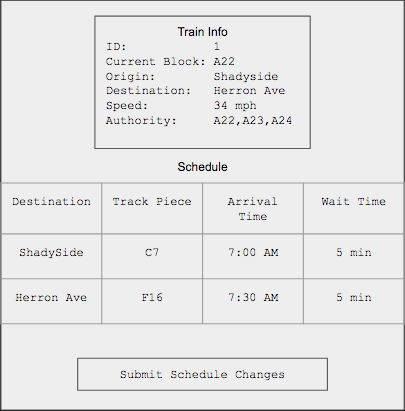
\includegraphics[width=10cm]{CTC-pop}
\end{center}
% trim={<left> <lower> <right> <upper>}
The same train information that was displayed in the main GUI will be replicated here. In
addition the train's individual schedule can be seen here and edited while in manual mode.

%%%%%%%%%%%%%%%%%%   CTC End   %%%%%%%%%%%%%%%%%%%%%

%%%%%%%%%%%%%%%%%%   WC Begin  %%%%%%%%%%%%%%%%%%%%%

\chapter{Wayside / Track Controller}
\Large{Isaac Goss}\\
\begin{center}
    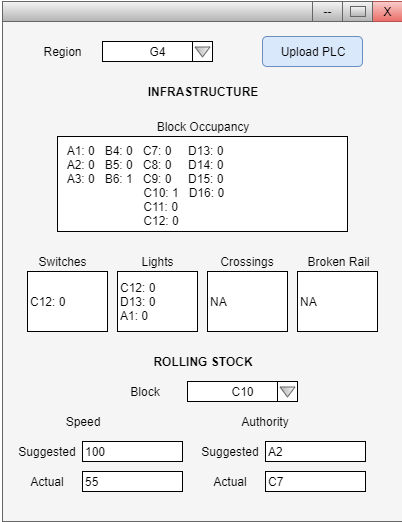
\includegraphics[width=0.5\textwidth]{wc-ui}
\end{center}



\section{Top Level}
\begin{center}
    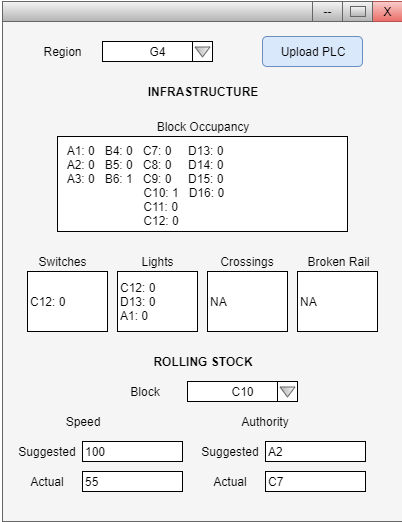
\includegraphics[trim = {.0 7.7cm 0cm 0cm }, clip, width=0.5\textwidth]{wc-ui}
\end{center}

\subsection{Region Selector}
This is a drop-down menu which allows the user to pick with which Wayside Controller (WC) she would like to interact.
The regions define a WC's subset of track which it controls, so this uniquely identifies a WC.
The region is specified by line (Green or Red), and the number within that line.

\subsection{Upload PLC}
Beside this, we see a button labeled "Upload PLC" which allows a user to change which PLC file this WC will execute.
Hitting this button will open a file menu to allow easy file choice.
If the upload and compilation of the PLC code is successful, the user will be returned to the main window.
However, if the upload fails in reading the file, or with an error in the code, the user will be presented with an error pop-up.

\begin{center}
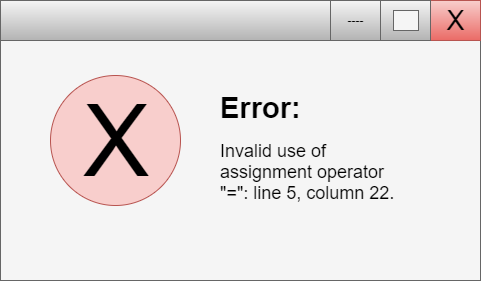
\includegraphics[width=0.4\textwidth]{wc-error}
\end{center}




\section{Infrastructure}
\begin{center}
    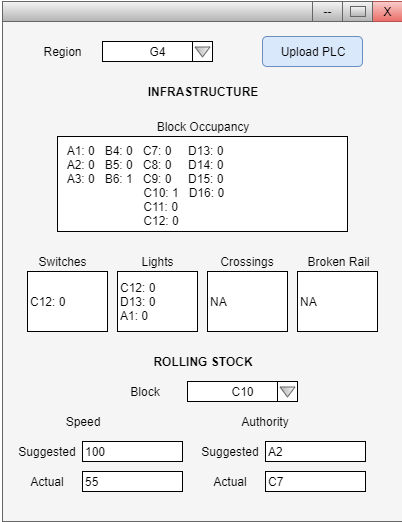
\includegraphics[trim = {0cm 3cm 0cm 1.3cm }, clip, width=0.5\textwidth]{wc-ui}
\end{center}


\subsection{Block Occupancy}
This view displays all blocks which this WC controls.
They are printed by name (section and number), followed by the binary value of occupancy: 1 if occupied, 0 otherwise.
It is automatically refreshed as this information changes.

\subsection{Switches, Lights, Crossings, and Broken Rail}
Each of these boxes work much like the Block Occupancy box above.
Information is presented by block number, in the same format, and each of these blocks will only print the relevant blocks, i.e., the only switch in this region is on C12, so only that block is printed.
The following additional information will be printed along with the block number, per box:

\begin{description}
    \item[Switches] Position, that is, whether the switch is engaged.
    \item[Lights] Color, from D (double green), G (green), Y (yellow), R (red).
    \item[Crossings] Whether a crossing is active, so that a train can pass over; 1 for activated, 0 for not activated.
    \item[Broken Rail] In maintenance; 0 for no (broken), 1 for yes.
\end{description}


\section{Rolling Stock}
\begin{center}
    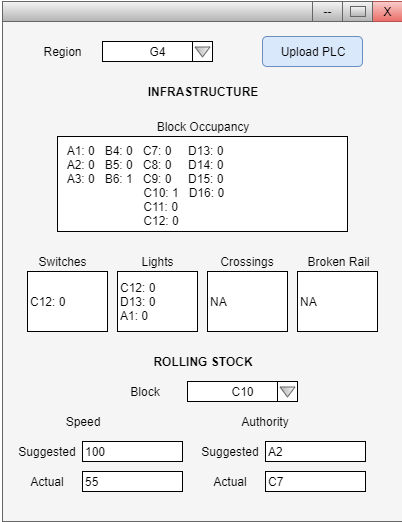
\includegraphics[trim = {0cm 0cm 0cm 6cm }, clip, width=0.5\textwidth]{wc-ui}
\end{center}

\subsection{Block}
This drop-down allows a user to pick the train to interact with by the block it is currently on.
This will be changing rapidly, but the drop-down menu will keep up with these changes to make selection painless.

\subsection{Speed}
Below, and to the left, there are 2 boxes, both of which represent some kind of speed assigned to this train. The first is \textbf{Suggested} Speed, which comes from the CTC.
As this is a vital component, the WC shall not allow this speed to exceed the speed limit of the train's current block.
This is called \textbf{Actual} Speed, and is what the WC assigns to the train in question.
These speeds shall be in miles per hour.

\subsection{Authority}
To the right of this, there are 2 very similar boxes.
These represent the Authority which was \textbf{Suggested} by the CTC, and the \textbf{Actual} Authority assigned by the WC controller.
The WC shall not allow a trains authority to exceed where it can safely go.
That is, the WC shall not allow a trains authority to overlap with any of the following:

\begin{enumerate}
    \item That of another train.
    \item A switch which a train cannot use at that time.
    \item A railroad crossing which it cannot cross at this time.
    \item Rail which it cannot use at this time.
\end{enumerate}


%%%%%%%%%%%%%%%%%%    WC End   %%%%%%%%%%%%%%%%%%%%%

\chapter{Track Model}
\Large{Alec Rosenbaum}\\
% picture(s) of overall gui
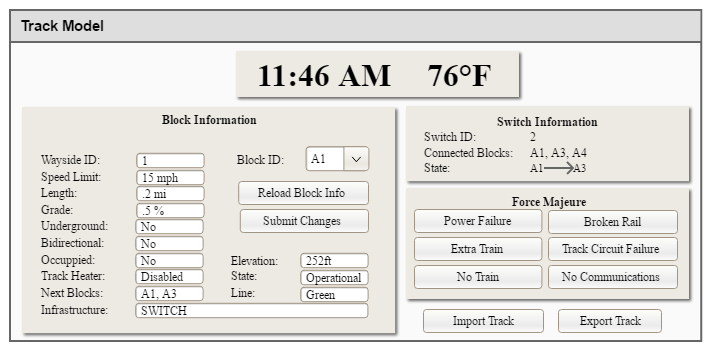
\includegraphics[width=\textwidth]{track-model}

\section{Block Information}

\begin{center}
    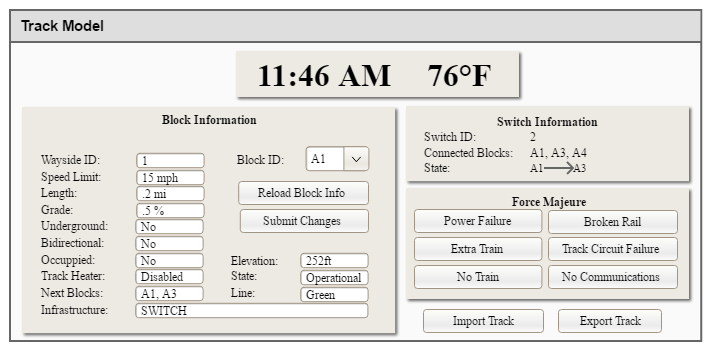
\includegraphics[trim={.5cm .5cm 11cm 3.6cm},clip,width=7.5cm]{track-model}
    % trim={<left> <lower> <right> <upper>}
\end{center}

The block information section allows the user to select a block (from a dropdown), view
stored block details, and reconfigure block details. Once the user selects a block from the
dropdown, that blocks information will be populated onto the appropriate fields. The user may
then reload the information about that block using the "Reload Block Info" button, or they
may edit any field and click the "Submit Changes" button to modify the details stored by
the Track Model.

The user may expect to see one or more of the following block states in the "State" field:
\begin{description}
    \item[Operational] The selected block is fully functional.
    \item[Broken Rail] The selected block includes a section of broken rail.
    \item[Extra Train] The selected block detects a train, when there is no train
        actually present.
    \item[No Train] The selected block does not detect a train, when a train is present.
    \item[Power Failure] The selected block is experiencing a power failure.
    \item[No Communication] The selected block's communications aren't functional, thus no
        communication is relayed to any train present.
\end{description}

\section{Switch Information}

\begin{center}
    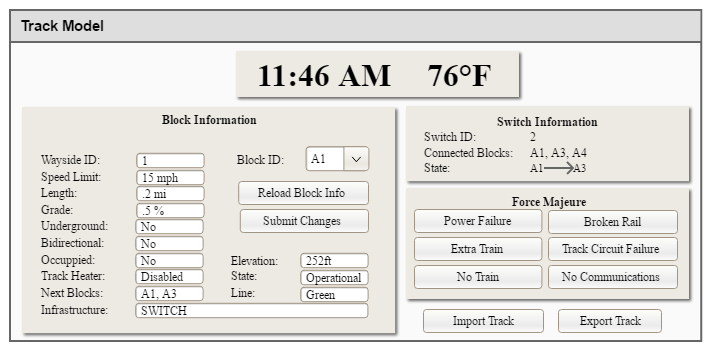
\includegraphics[trim={14.2cm 5.75cm .5cm 3.6cm},clip,width=6cm]{track-model}
    % trim={<left> <lower> <right> <upper>}
\end{center}

If there is a switch connected to the selected block, details will be presented in
this section. Details include:
\begin{itemize}
    \item Switch ID
    \item Connected Blocks
    \item Switch State
\end{itemize}

\section{Force Majeure}

\begin{center}
    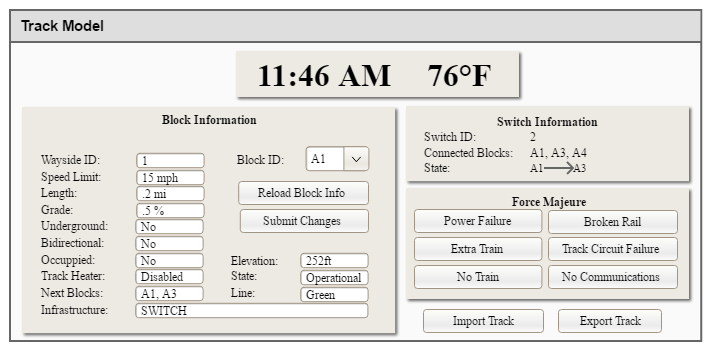
\includegraphics[trim={14.2cm 1.75cm .5cm 6.5cm},clip,width=7.5cm]{track-model}
    % trim={<left> <lower> <right> <upper>}
\end{center}

All options for causing Force Majeure failures are presented here. When the user clicks
an option, the Force Majeure failure is applied to the selected block.

\section{Track Import and Export}

\begin{center}
    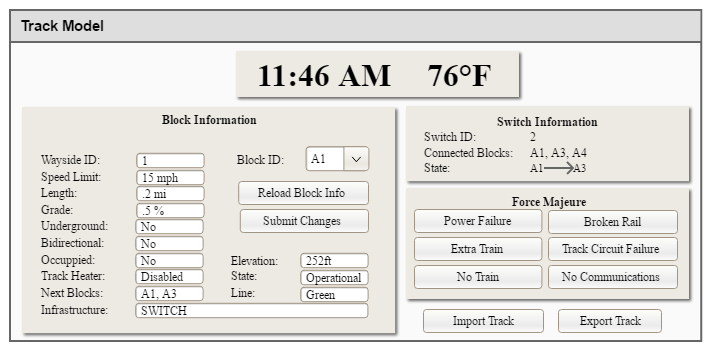
\includegraphics[trim={14.2cm .5cm .5cm 10.75cm},clip,width=7.5cm]{track-model}
    % trim={<left> <lower> <right> <upper>}
\end{center}

Track import and export options are presented here. The "Import Track" button allows
the entire track to be replaced with an imported track. The "Export Track" button allows
the entire track to be exported based on its current state.

%%%%%%%%%%%%%%%%%%   Train Model   %%%%%%%%%%%%%%%%%%%%%
\chapter{Train Model}
\Large{Parth Dadhania}\\
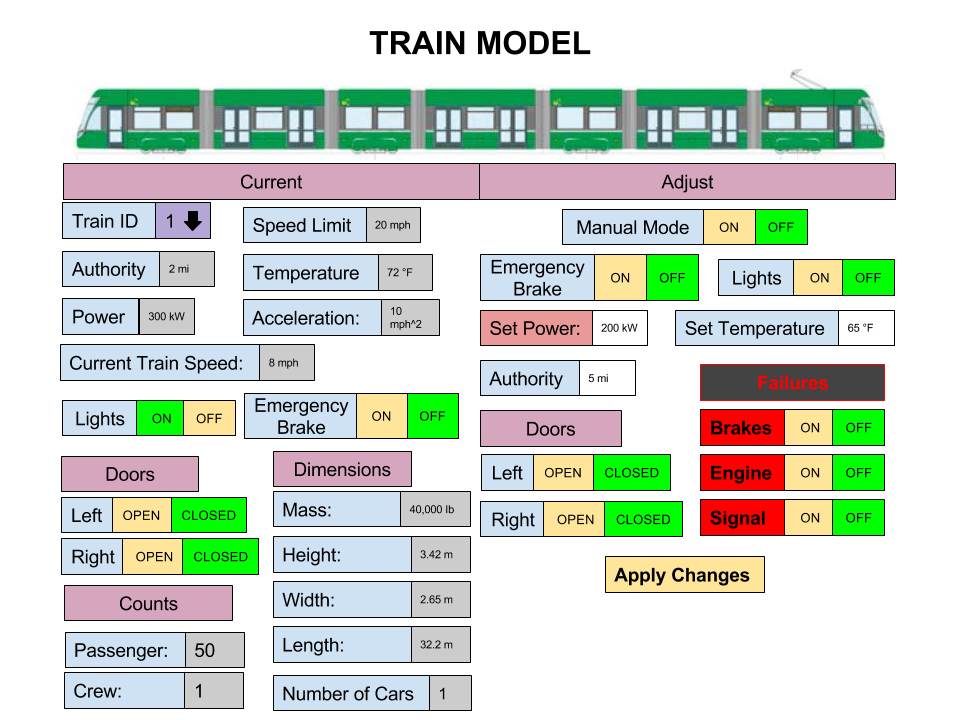
\includegraphics[width=\textwidth]{TrainModelUI}

\section{Current}
\begin{itemize}
    \item Train Id: Drop down to let user select a train
    \item Speed Limit: Displays the current speed limit
    \item Authority: Displays the current authority
    \item Temperature: Displays the current temperature inside the train
    \item Power: Displays the current power
    \item Acceleration: Displays the current acceleration of the train
    \item Current Train Speed: Displays the speed of the train
    \item Lights: Displays the current status of the headlights
    \item Emergency Brake: Displays current status of the emergency brakes
    \item Doors: Displays the status of the left and right doors on the train
    \item Passengers: Displays the number of passengers on the train
    \item Crew: Displays the number of crew members on the train
\end{itemize}

\section{Dimensions}
\begin{itemize}
    \item Mass: Displays the mass of the train
    \item Height: Displays the height of the train
    \item Width: Displays the width of the train
    \item Length: Displays the length of the train
    \item Number of Cars: Displays the number of cars for
\end{itemize}

\section{Adjust}

\begin{itemize}
    \item Manual Mode: Select ON to adjust specific aspects of the train
    \item Emergency Brake: Select ON to engage emergency brakes
    \item Lights: Lets user turn on and off the train's headlights
    \item Power: User can set power input
    \item Temperature: User can set inside temperature for the train
    \item Authority: User can set authority of the train
    \item Doors: User can open or close the doors on the left and right side
    \item Failures: Users can turn on and off failures that could occur in the train
    \item Apply Changes: Submits the inputs that the user provided in the fields above
    \end{itemize}
%%%%%%%%%%%%%%%%%%  End Train Model   %%%%%%%%%%%%%%%%%%%%%


%%%%%%%%%%%%%%%  Begin Train Controller  %%%%%%%%%%%%%%%%%%
\chapter{Train Controller}
\Large{Aric Hudson}\\\\
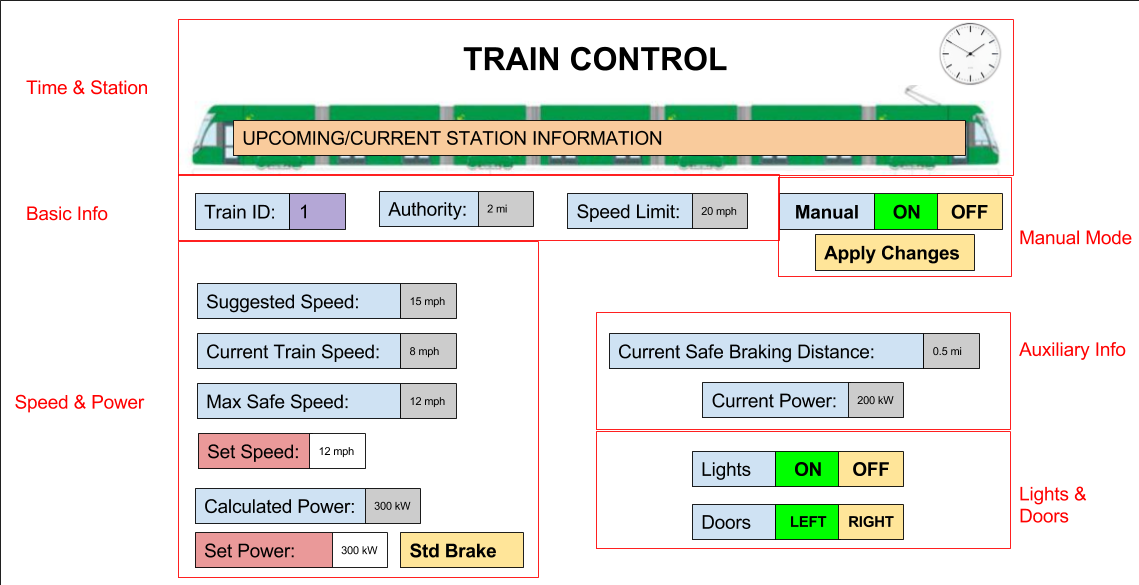
\includegraphics[width=\textwidth]{tc}

\section{Time \& Station}
\begin{itemize}
    \item Upcoming and Current Station Information: Displays the next station or the current station if stopped at one.
    \item Clock Icon: displays the current time, and speed of simulation
\end{itemize}

\section{Basic Info}
\begin{itemize}
    \item Train ID: Displays ID of current train; dropdown menu allows user to view different trains.
    \item Authority: Displays current train's authority in miles.
    \item Speed Limit: displays the current speed limit the train is under, if it knows what that speed limit is.
\end{itemize}

\section{Speed \& Power}
\begin{itemize}
    \item Suggested Speed: Speed suggested for the train by the Wayside Controller.
    \item Current Train Speed: Current speed of the train currently being viewed.
    \item Max Safe Speed: Maximum safe speed for train as calculated by Train Controller.
    \item Set Speed: Speed to set train to; can be dictated in manual mode; updated automatically in automatic mode.
    \item Calculated Power: The necessary power required by the train to attain the desired speed. Will display "brake" if the train needs to slow down.
    \item Set Power: Power to set the train to; can be dictated in manual mode; updated automatically in automatic mode.
    \item Std Brake: Applies the regular brake to the system as long as it is held.
\end{itemize}

\section{Manual Mode}
\begin{itemize}
    \item Manual: Toggles manual mode when "ON" is selected; toggles automatic mode when "OFF" is selected.
    \item Apply Changes: When manual changes have been set, this applies the changes to the current train.
\end{itemize}

\section{Auxiliary Info}
\begin{itemize}
    \item Current Safe Braking Distance: The current safe braking distance as calculated by train controller.
    \item Current Power: The current power applied to the train.
\end{itemize}

\section{Lights \& Doors}
\begin{itemize}
    \item Lights: Toggles lights on or off.  Lights should be on when "ON" is toggled; lights should be off when "OFF" is toggled.
    \item Doors: Toggles doors to open.  If doors on left are open, toggling "LEFT" closes them; if the doors on the left are closed, toggling "LEFT" opens them.  The "RIGHT" toggle has identical functionality, but for the right doors.
\end{itemize}


%%%%%%%%%%%%%%%%% End Train Controller %%%%%%%%%%%%%%%%%%%%%%
\end{document}
